\documentclass{../TexTemplate/myslide}
\usepackage[slide,table,cpp]{../TexTemplate/mypackage}
\hypersetup{colorlinks=true,linkcolor=black,urlcolor=blue}
\usepackage{xcolor}

\renewcommand{\thefootnote}{\fnsymbol{footnote}}

\title[ToolsSeminar]{Tools Seminar}
\subtitle{Week 10 - Parallel Computing}
\author[chhzh123]{Hongzheng~Chen}
\date[Apr 25, 2020]{Apr 25, 2020}

\begin{document}
% GPU CUDA

\begin{frame}
\titlepage
\end{frame}

\begin{frame}
\tableofcontents
\end{frame}

% https://chhzh123.github.io/summary/parallel-computing/
\section{Introduction}
\begin{frame}
\sectionpage
\end{frame}

\begin{frame}
\begin{figure}
\centering
\includegraphics[width=\linewidth]{fig/the_end_of_moores_law_and_scaling.png}
\end{figure}
* That's why \href{https://en.wikipedia.org/wiki/Tick\%E2\%80\%93tock_model}{Intel} is called ``toothpaste factory'' now
% http://blog.peddy.ai/2019/04/03/evolution-of-hardware-for-deep-learning/
\end{frame}

\begin{frame}{The End of Moore's Law and Scaling}
\begin{quote}
This shift toward \textbf{increasing parallelism} is not a triumphant stride forward based on breakthroughs in novel software and architectures for parallelism;
instead, this plunge into parallelism is actually a \textbf{retreat} from even greater challenges that thwart efficient silicon implementation of traditional uniprocessor architectures.\\
\hfill ---  \emph{The Landscape of Parallel Computing Research: A View from Berkeley}, 2006
\end{quote}
\pause
\begin{itemize}
\item All the CPUs now have multiple cores, so the system always works in parallel!
\item Multicore processors put burdens from hardware to software, which needs programmers to code \textbf{parallel programs}.
\end{itemize}
\end{frame}

\begin{frame}{Parallel Computing}
Tightly associated with scientific computing (big data!)
\begin{itemize}
	\item Computational biology (gene, protein)
	\item Weather/Climate prediction
	\item Ocean circulation
	\item Astronomy
	\item Material
	\item Physics
\end{itemize}
Supercomputer itself is a highly distributed parallel architecture
\end{frame}

\begin{frame}{Supercomputing}
\begin{figure}[H]
\centering
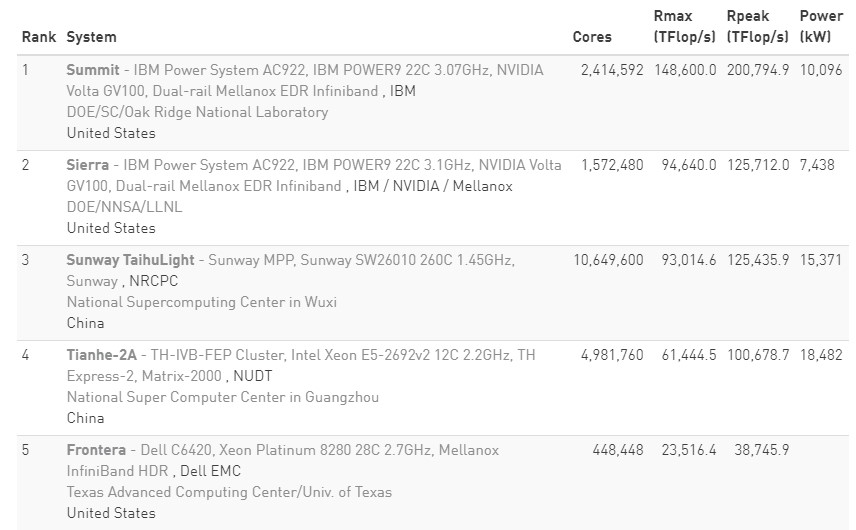
\includegraphics[width=0.8\linewidth]{fig/top500.jpg}
\caption*{\href{https://www.top500.org/lists/2019/11/}{Top 500} List November 2019}
\end{figure}
\end{frame}

\begin{frame}{Different hardware}
\begin{figure}[H]
\centering
\includegraphics[width=0.8\linewidth]{fig/accelerator_comparison.png}
\end{figure}
\begin{itemize}
	\item CPU (Central Processing Unit): Intel, AMD, Arm
	\item GPU (Graphical Processing Unit): Intel, Nvidia
	\item FPGA (Field-Programmable Gate Array): Intel (Altera), Xilinx
	\item ASIC (Application-Specific Integrated Circuit): Intel, Samsung, Quantum, Hisilicon
\end{itemize}
\end{frame}

\begin{frame}{Von Neumann Architecture}
\begin{figure}
\centering
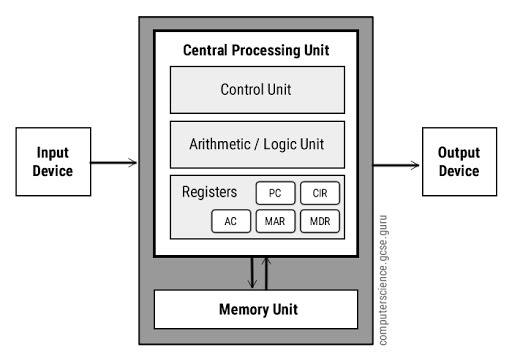
\includegraphics[width=0.6\linewidth]{fig/von-neumann.jpg}
\end{figure}
\end{frame}

\begin{frame}{CPU Architecture}
\begin{figure}
\centering
\includegraphics[width=0.9\linewidth]{fig/Intel-core-i7-cpu-die.jpg}
\caption*{\small Intel core i7 CPU (Ivy Bridge)}
% https://www.anandtech.com/Show/Index/5771?cPage=10&all=False&sort=0&page=3&slug=the-intel-ivy-bridge-core-i7-3770k-review
\end{figure}
* See CSAPP
\end{frame}

\begin{frame}
\begin{figure}
\centering
\includegraphics[width=\linewidth]{fig/gpu-fpga.jpg}
\end{figure}
\small
\begin{itemize}
\item CPU \& GPU: Traditional von Neumann architecture with instruction interpretation overheads
\item FPGA: Directly program \textbf{circuits}!
\end{itemize}
\pause
We will focus on CPU parallelism in this seminar
\end{frame}

\begin{frame}{Shared-Memory \& Distributed-Memory}
\begin{figure}[H]
\centering
\begin{tabular}{cc}
Shared-memory & 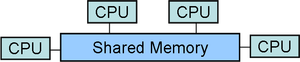
\includegraphics[width=0.5\linewidth]{fig/shared-memory-model.png}\\
\quad & \quad\\
Distributed-memory & 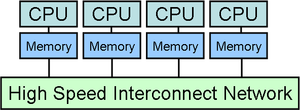
\includegraphics[width=0.5\linewidth]{fig/distributed_memory_model.png}
\end{tabular}
\caption*{\small Fig source: \href{https://bioinfomagician.wordpress.com/2013/11/11/parallel-computing-introduction-to-mpi/}{Parallel Computing: Introduction to MPI}}
\end{figure}
\end{frame}

\section{Shared-Memory Parallelism}
\begin{frame}
\sectionpage
\end{frame}

\begin{frame}[fragile]{Check your CPU}
See how many CPU cores do you have
\begin{itemize}
\item Windows: Open the task manager
\item Linux: \verb'lscpu'
\end{itemize}
\end{frame}

\subsection{Multi-threads}
\begin{frame}
\subsectionpage
\end{frame}

\begin{frame}[fragile]{Process \& Thread}
Check \verb'top'. Commonly, one program is a process.
\begin{figure}
\centering
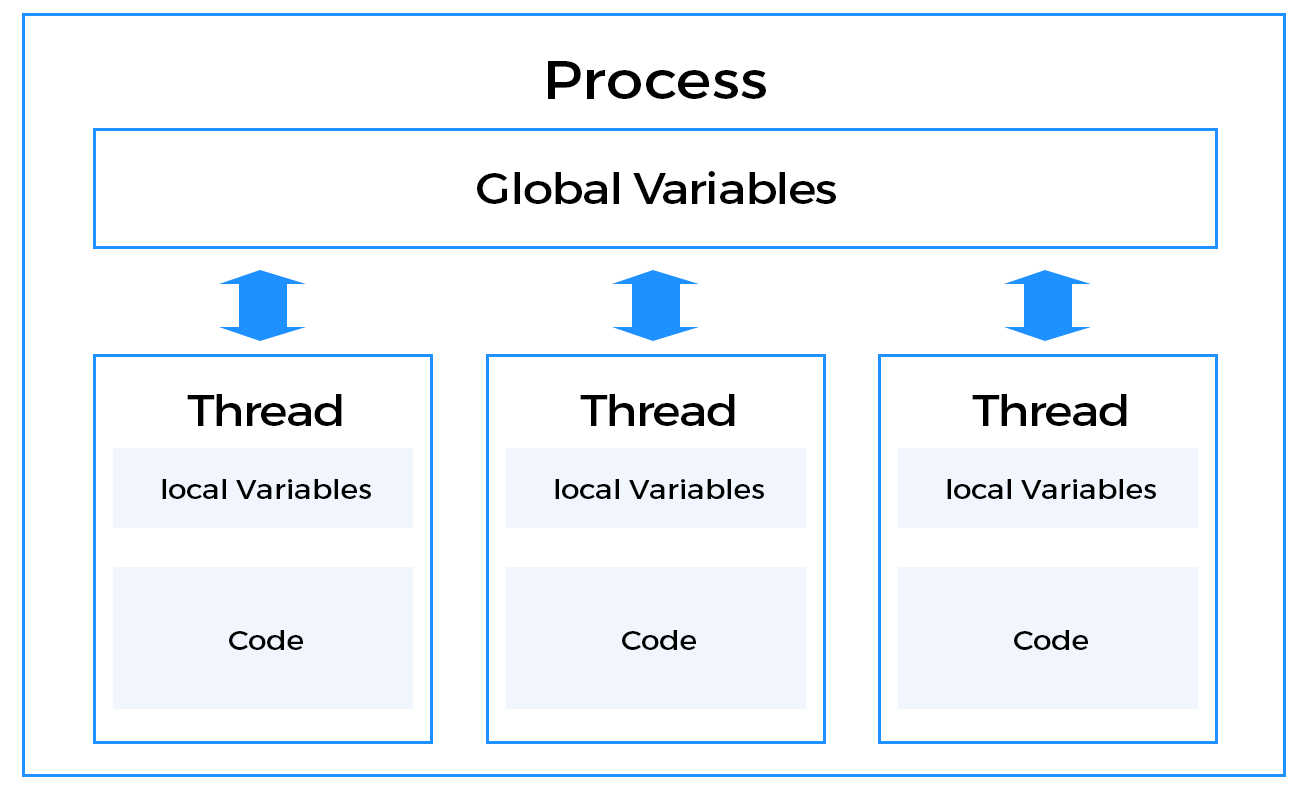
\includegraphics[width=0.8\linewidth]{fig/process_thread.png}
\caption*{\small \href{https://www.educative.io/courses/java-multithreading-for-senior-engineering-interviews/m2G48X18NDO}{Multi-threading}}
\end{figure}
\end{frame}

\begin{frame}{Fork-Join Model}
\begin{figure}
\centering
\includegraphics[width=\linewidth]{fig/fork-join.png}
\end{figure}
\begin{itemize}
	\item Fork: Dispatch tasks to each processor / thread
	\item Join: Synchronization, wait till all threads are done
\end{itemize}
\end{frame}

% https://chhzh123.github.io/blogs/2019-03-14-cpp-multithreading/
\begin{frame}[fragile]{pthread}
\href{https://en.wikipedia.org/wiki/POSIX_Threads}{POSIX} (Portable Opearing System Interface for Unix)
\begin{itemize}
\item \verb'<pthread.h>' is in Linux's system library and can be directly called
\end{itemize}
\begin{lstlisting}[basicstyle=\scriptsize]
void *foo(void *arg)
{
	int* id = (int*) arg;
	printf("My id is %d\n", *id);
}

int main()
{
	pthread_t id[4];
	for (int i = 0; i < 4; ++i)
		// pass in function pointer and args
		pthread_create(&id[i],NULL,foo,&i);
	for (int i = 0; i < 4; ++i)
		pthread_join(&id[i],NULL);
	for (int i = 0; i < 4; ++i)
		pthread_exit(&id[i]);
}
\end{lstlisting}
Need to add \verb'-lpthread' flag when compiling
\end{frame}

\begin{frame}[fragile]{C++11 thread}
C++11 adds initial support for multi-threading in stl
\begin{lstlisting}
#include <iostream>
#include <thread>
using namespace std;

void exec(int n){
	cout << "My id is" << n << endl;
}

int main(){
	thread myThread[4];
	for (int i = 0; i < 4; ++i)
		myThread[i] = thread(exec,i);
	for (int i = 0; i < 4; ++i)
		myThread[i].join();
}
\end{lstlisting}
\end{frame}

\begin{frame}{Race Condition}
Be careful of the shared data
\begin{center}
\begin{tabular}{c|c}
Thread A & Thread B\\
$\cdots$ & $\cdots$\\
Count$++$ & Count$--$\\
$\cdots$ & $\cdots$
\end{tabular}\quad
\begin{tabular}{ll|ll}
Thread A & & Thread B\\
Load & Count & Load & Count\\
Add & \#1 & Sub & \#1\\
Store & Count & Store & Count
\end{tabular}
\end{center}
\begin{itemize}
	\item Critical section: That part of the program where the shared memory is accessed
	\item Need to avoid conflicts and make data consistent
\end{itemize}
\end{frame}

\begin{frame}{Avoid Race Condition}
Two basic methods:
\begin{itemize}
	\item Corse-grained: Lock/mutex
	\item Fine-grained: Atomic operations
\end{itemize}
* There are lots of details about synchronization \& consistency, please refer to books of OS
\end{frame}

\begin{frame}[fragile]{Mutex Operations in pthread}
\verb'<pthread.h>'
\begin{itemize}
\item \verb'pthread_mutex_init(&mutex1,NULL)'
\item \verb'pthread_mutex_destroy(&mutex1)'
\item \verb'pthread_mutex_lock(&mutex1)'
\item \verb'pthread_mutex_unlock(&mutex1)'
\end{itemize}
\verb'<thread>'
\begin{itemize}
	\item \verb'std::mutex g_display_mutex'
	\item \verb'std::lock_guard<std::mutex> guard(g_display_mutex)'
\end{itemize}
\end{frame}

\begin{frame}[fragile]{Multi-threading in Python}
\begin{itemize}
	\item \verb'threading.Thread'
	\item \verb'multiprocessing.Process'
	\item \verb't1.start()', \verb't1.join()'
	\item \href{https://en.wikipedia.org/wiki/Global_interpreter_lock}{Global Interpreter Lock} (GIL) limitation $\to$ CPython
	\begin{quote}
	An interpreter that uses GIL always allows exactly one thread to execute at a time, even if run on a multi-core processor.
	\end{quote}
\end{itemize}
Ref: \url{https://realpython.com/intro-to-python-threading/}
\end{frame}

\subsection{OpenMP}
\begin{frame}
\subsectionpage
\end{frame}

% https://chhzh123.github.io/summary/parallel-computing/openmp/
\begin{frame}{OpenMP}
\href{https://www.openmp.org/}{OpenMP} (Open Multi-Processing): Shared-memory programming model
\begin{itemize}
	\item Set of parallel commands, library, and routines
	\item Simplify multi-threading programming
	\item A spec suitable for different devices from desktop to supercomputer
	\item gcc has initial support for OpenMP
\end{itemize}
\end{frame}

\begin{frame}[fragile]{OpenMP API}
\verb'#include <omp.h>' and only need to write compilation directives
\begin{center}
\verb'#pragma omp <directive-name> [clause,...]'
\end{center}
\begin{itemize}
	\item \verb'omp_get_thread_num'
	\item \verb'omp_get/set_num_procs'
	\item \verb'omp_get/set_num_threads'
	\item \verb'#pragma omp parallel for': The most commonly used!
	\item \verb'#pragma omp ... private (<variable list>)'
	\item \verb'#pragma omp ... reduction (op:list)'
\end{itemize}
\end{frame}

\begin{frame}[fragile]{OpenMP Example (Matrix Multiplication)}
\begin{lstlisting}
#pragma omp parallel num_threads(8)
for (int i = 0; i < m; ++i)
  for (int j = 0; j < n; ++j) {
    c[i][j] = 0.0;
    for (int k = 0; k < l; ++k)
      c[i][j] += a[i][j] * b[j][k];
  }
\end{lstlisting}
Compile with \verb'-fopenmp'
\end{frame}

\begin{frame}[fragile]{OpenMP Example (Summation)}
\begin{lstlisting}
float sum(const float *a, size_t n)
{
    float total = 0.;

    #pragma omp parallel for reduction(+:total)
    for (size_t i = 0; i < n; i++) {
        total += a[i];
    }
    return total;
}
\end{lstlisting}
\end{frame}

\subsection{Cilk Plus}
\begin{frame}
\subsectionpage
\end{frame}

% https://chhzh123.github.io/summary/parallel-computing/cilk/
\begin{frame}[fragile]{Intel Clik Plus}
\href{https://www.cilkplus.org/}{Intel Cilk Plus}: A extremely light-weighted parallel framework
\begin{itemize}
	\item \verb'#include<cilk/cilk.h>'
	\item gcc 5.0+: \verb'g++ -O3 -fcilkplus -lcilkrts <source>'
	\item Or compiled by Intel Compiler (icpc) --- Better choice!
	\begin{itemize}
		\item But from icpc 18.0, Intel uses \href{https://software.intel.com/en-us/articles/migrate-your-application-to-use-openmp-or-intelr-tbb-instead-of-intelr-cilktm-plus?_ga=2.174275746.1279103381.1550824040-508775473.1544510410}{Thread Building Block} (TBB)
	\end{itemize}
\end{itemize}
Only three keywords
\begin{itemize}
	\item \verb'cilk_spawn': fork
	\item \verb'cilk_sync': join
	\item \verb'cilk_for': \verb'parallel for'
\end{itemize}
\end{frame}

\begin{frame}[fragile]{Clik Example (Fibbonacci)}
\begin{lstlisting}
int fib(int n)
{
    if (n < 2)
        return n;
    int x = fib(n-1);
    int y = fib(n-2);
    return x + y;
}

int fib(int n)
{
    if (n < 2)
        return n;
    int x = cilk_spawn fib(n-1);
    int y = fib(n-2);
    cilk_sync;
    return x + y;
}
\end{lstlisting}
\end{frame}

\begin{frame}{Cilk Runtime}
The most powerful thing is Cilk runtime deploys \textbf{work-stealing} scheduling strategy, which greatly outperforms OpenMP's runtime
\begin{figure}[H]
\centering
\includegraphics[width=0.7\linewidth]{fig/tbb.png}
\caption*{\small Fig source: \href{https://csdl-images.computer.org/mags/so/2011/01/figures/mso20110100232.gif}{Intel TBB}}
\end{figure}
\end{frame}

\subsection{Finer-grained Parallelism}
\begin{frame}
\subsectionpage
\end{frame}

\begin{frame}{Parallelism}
\begin{itemize}
	\item Thread-Level Parallelism (TLP)
	\item Instruction-Level Parallelism (ILP)
	\begin{itemize}
		\item Pipelining
		\item Hyperscalar
		\item Very Long Instruction Word (VLIW)
		\item Vector processing
		\item Out-of-Order (OoO) execution
		\item Spectacular execution
	\end{itemize}
	\item Data-Level Parallelism
	\begin{itemize}
		\item SIMD (Single Instruction Multiple Data) array processor $\to$ GPU
	\end{itemize}
\end{itemize}
% https://www.archive.ece.cmu.edu/~ece740/f13/lib/exe/fetch.php?media=seth-740-fall13-module5.1-simd-vector-gpu.pdf
* Please refer to Computer Architecture books / CSAPP
\end{frame}

\begin{frame}{SIMD}
\begin{figure}
\centering
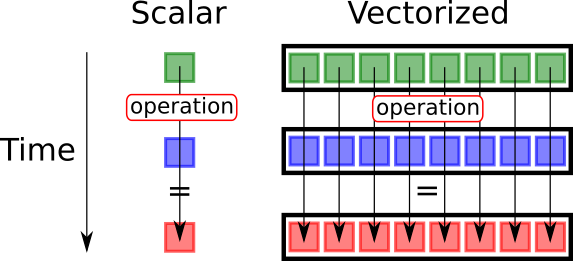
\includegraphics[width=0.8\linewidth]{fig/vectorization.png}
\caption*{\small Fig source: \url{https://lappweb.in2p3.fr/~paubert/ASTERICS_HPC/6-6-1-985.html}}
\end{figure}
\end{frame}

% https://chhzh123.github.io/blogs/2019-03-03-AVX/
\begin{frame}{Intel CPU SIMD Instruction Set}
\begin{itemize}
	\item MME (Multi Media Extensions): Pentium, 1996
	\item SSE (Streaming SIMD Extensions): Pentium III, 1999
	\item AVX (Advanced Vector Extensions): Sandy Bridge 2008
	\item AVX2: Haswell, 2011
\end{itemize}
\end{frame}

\begin{frame}[fragile]{Naming Conventions}
\verb'_mm<bit_width>_<name>_<data_type>'
\begin{itemize}
\item \verb'<bit_width>': the return size, 128 - empty, 256 - 256
\item \verb'<name>': describes the operation performed by the intrinsic
\item \verb'<data_type>': the function's primary arguments
\end{itemize}
\begin{center}
\begin{tabular}{cc}\hline
Instructions & Description\\\hline
ps &	packed single-precision\\
pd &	packed double-precision\\
epi8/epi16/epi32/epi64 &	signed integers\\
epu8/epu16/epu32/epu64 &	unsigned integers\\
si128/si256 &	unspecified vector\\
m128/m128i/m128d &	input vector types\\\hline
\end{tabular}
\end{center}
e.g. \verb'_mm256_srlv_epi64':  64-bit signed int $\to$ 256-bit vector
\end{frame}

\begin{frame}[fragile]{AVX Example}
\begin{lstlisting}[basicstyle=\scriptsize]
#include <immintrin.h>
#include <stdio.h>

int main() {

    /* Initialize the two argument vectors */
    __m256 evens = _mm256_set_ps(2.0, 4.0, 6.0, 8.0, 10.0, 12.0, 14.0, 16.0);
    __m256 odds = _mm256_set_ps(1.0, 3.0, 5.0, 7.0, 9.0, 11.0, 13.0, 15.0);

    /* Compute the difference between the two vectors */
    __m256 result = _mm256_sub_ps(evens, odds);

    /* Display the elements of the result vector */
    float* f = (float*) &result; // type conversion
    printf("%f %f %f %f %f %f %f %f\n",
      f[0], f[1], f[2], f[3], f[4], f[5], f[6], f[7]);

    return 0;
}
\end{lstlisting}
Add \verb'-mavx' flag when compiling\\
* Be careful that redundant movements reduce performance!
\end{frame}

\section{Distributed-Memory Parallelism}
\begin{frame}
\sectionpage
\end{frame}

% https://chhzh123.github.io/summary/parallel-computing/mpi/
\begin{frame}[fragile]{Message Passing Interface (MPI)}
\begin{itemize}
\item All the machine execute the \textbf{same} program!
\item Use condition to judge whether it needs to execute this piece of code
\item Need to install \href{http://www.mpich.org/}{MPI} compiler
\begin{itemize}
	\item \verb'#include<mpi.h>'
	\item \verb'mpicc', \verb'mpic++'
	\item \verb'mpirun -np 2 foo : -np 4 bar'
\end{itemize}
\end{itemize}
\end{frame}

\begin{frame}{Distributed Memory Model}
\begin{figure}
\centering
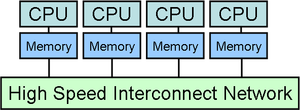
\includegraphics[width=0.5\linewidth]{fig/distributed_memory_model.png}
\caption*{Each host has a rank}
\end{figure}
* Tianhe2 with millions of distributed nodes need to explicitly manage communication via MPI
\end{frame}

\begin{frame}[fragile]{MPI Hello World}
\begin{lstlisting}
#include <mpi.h>

int main(int argc, char* argv[])
{
    int npes, myrank;
    MPI_Init(&argc, &argv);
    MPI_Comm_size(MPI_COMM_WORLD, &npes);
    MPI_Comm_rank(MPI_COMM_WORLD, &myrank);
    printf("From process %d out of %d, Hello World!\n", myrank, npes);
    MPI_Finalize();
}
\end{lstlisting}
\end{frame}

\begin{frame}[fragile]{Message Passing}
Message communication is the central part of MPI
\begin{lstlisting}[basicstyle=\scriptsize]
MPI_Send(
    void* data,
    int count,
    MPI_Datatype datatype,
    int destination,
    int tag,
    MPI_Comm communicator)

MPI_Recv(
    void* data,
    int count,
    MPI_Datatype datatype,
    int source,
    int tag,
    MPI_Comm communicator,
    MPI_Status* status)
\end{lstlisting}
\end{frame}

\begin{frame}[fragile]{MPI Example Program (Ping Pong)}
\begin{lstlisting}
int ping_pong_count = 0;
int partner_rank = (world_rank + 1) % 2;
while (ping_pong_count < PING_PONG_LIMIT) {
    if (world_rank == ping_pong_count % 2) {
        // Increment the ping pong count before you send it
        ping_pong_count++;
        MPI_Send(&ping_pong_count, 1, MPI_INT, partner_rank, 0,
                 MPI_COMM_WORLD);
        printf("%d sent and incremented ping_pong_count "
               "%d to %d\n", world_rank, ping_pong_count,
               partner_rank);
    } else {
        MPI_Recv(&ping_pong_count, 1, MPI_INT, partner_rank, 0,
                 MPI_COMM_WORLD, MPI_STATUS_IGNORE);
        printf("%d received ping_pong_count %d from %d\n",
               world_rank, ping_pong_count, partner_rank);
    }
}
\end{lstlisting}
\end{frame}

\section{Parallel Computing Frameworks}
\begin{frame}
\sectionpage
\end{frame}

% https://chhzh123.github.io/summary/parallel-computing/mapreduce/
% https://chhzh123.github.io/summary/parallel-computing/spark/
\begin{frame}{Frameworks}
\begin{figure}
\centering
\includegraphics[width=0.6\linewidth]{fig/mapreduce.png}
\end{figure}
\begin{itemize}
\item \href{https://www.tutorialspoint.com/hadoop/hadoop_mapreduce.htm}{MapReduce}: Big data programming model $\to$ Hadoop
\item \href{https://spark.apache.org}{Spark}: Better data management
\item \href{https://rise.cs.berkeley.edu/projects/ray/}{Ray}: Machine Learning
\end{itemize}
\end{frame}

\section{Summary}
\begin{frame}
\sectionpage
\end{frame}

\begin{frame}{Summary}
\begin{itemize}
	\item Introduction to parallelism
	\item Shared-memory: pthreads, OpenMP, Cilk, AVX
	\item Distributed-memory: MPI
	\item Parallel computing frameworks: MapReduce
\end{itemize}
\end{frame}

\end{document}